\section{Tổ chức, truy vấn và biến đổi dữ liệu}
\label{sec:data-processing}

Mục này mô tả cách dữ liệu đi từ các file text gốc đến bảng đầu vào của mô hình,
theo các câu hỏi về cách gom nhiều file, lưu trữ, truy vấn và biến đổi dữ liệu,
qua những bước nào, dùng những cột nào, và các bảng quan hệ với nhau ra sao.
Hình~\ref{fig:data-flow} tóm tắt toàn bộ luồng; mỗi hộp là một bảng, ghi rõ một
dòng biểu diễn điều gì và kích thước thực tế với FD001. Mọi ví dụ trong mục này
có thể chạy lại từng bước trong notebook
\filepath{notebooks/00_data_pipeline_walkthrough.ipynb}; notebook gọi đúng các hàm
của pipeline và in kết quả trung gian.

Theo vòng đời quản lý dữ liệu của môn học, pipeline được ánh xạ trực tiếp thành
năm bước: \textbf{thu thập} các file C-MAPSS và lưu hash nguồn; \textbf{làm sạch}
bằng schema contract, kiểm tra khóa, cycle và giá trị hữu hạn, rồi khử nhiễu sensor
bằng EWMA; \textbf{chuẩn hóa} kiểu dữ liệu, tên cột, thứ tự khóa, và thang đo bằng
StandardScaler trước khi tạo Health Index; \textbf{tích hợp} train/test bằng UNION,
ghép nhãn theo khóa ba thành phần và tạo các bảng Silver--Gold; cuối cùng
\textbf{lưu trữ} thành Parquet và SQLite để truy vấn bằng Pandas, SQL hoặc
PySpark. Như vậy, mỗi bước đều có đầu vào, đầu ra và kiểm tra tương ứng thay vì
chỉ mô tả bước tạo đặc trưng.

\begin{figure}[H]
\centering
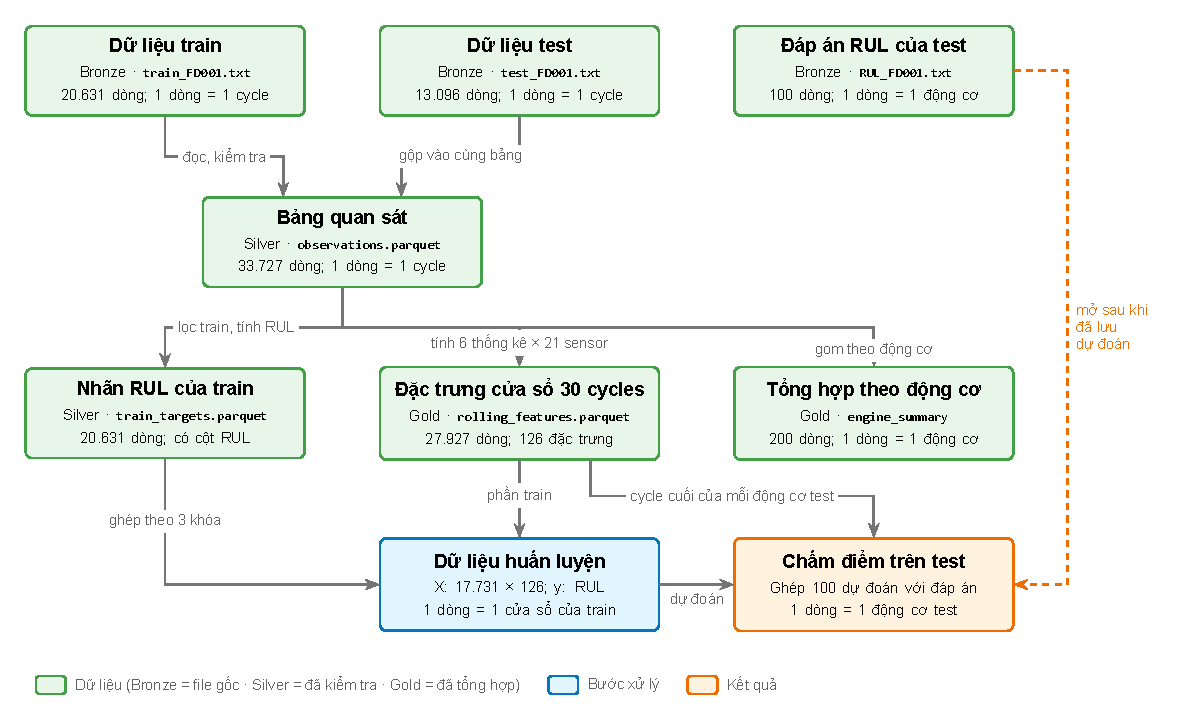
\includegraphics[width=0.97\linewidth]{figures/data-flow.pdf}
\caption[Luồng dữ liệu C-MAPSS]{Luồng dữ liệu từ ba file gốc đến dữ liệu huấn luyện và đánh giá cuối.
Chữ trên mũi tên là phép biến đổi; nhãn test chỉ được đọc sau khi dự đoán đã được ghi.}
\label{fig:data-flow}
\end{figure}

\subsection{Gom dữ liệu từ nhiều file}
\label{sec:dp-union}
Mỗi subset có ba file. Hai file quan sát \texttt{train\_FD001.txt} và
\texttt{test\_FD001.txt} có cùng 26 cột nhưng chứa hai nhóm động cơ khác nhau, nên
chúng được \textbf{nối theo chiều dòng (union)}, không phải join. Trước khi nối,
mỗi dòng được gắn thêm cột \texttt{split} để biết nó thuộc tập nào
(Mã nguồn~\ref{lst:union}). Bảng kết quả của FD001 có $20.631+13.096=33.727$ dòng
và 27 cột.

\begin{lstlisting}[language=Python,caption={Đọc và gom hai file quan sát (rút gọn từ
\texttt{pandas\_pipeline.py} và \texttt{spark\_pipeline.py}).},label={lst:union}]
# Pandas: read each file, validate 26 fields, add the split column, then union rows
frames = [read_observations(raw_dir / f"{split}_FD001.txt", split=split)
          for split in ("train", "test")]
observations = pd.concat(frames, ignore_index=True)
observations = observations.sort_values(["split", "engine_id", "cycle"])

# PySpark: the same union on Spark DataFrames
observations = train.unionByName(test).orderBy("split", "engine_id", "cycle")
\end{lstlisting}

Cột \texttt{split} là cần thiết vì train engine 1 và test engine 1 là hai động cơ
khác nhau nhưng có cùng \texttt{(engine\_id, cycle)}. Sau khi nối, cặp
\texttt{(engine\_id, cycle)} bị trùng, còn bộ ba \textbf{\texttt{(split, engine\_id,
cycle)}} là duy nhất; đây là khóa của mọi bảng ở cấp cycle. File nhãn
\texttt{RUL\_FD001.txt} không được gom vào bảng này mà được giữ riêng đến bước đánh
giá cuối. Bốn subset FD001--FD004 được xử lý ở bốn thư mục riêng; nếu muốn gộp
thành một bảng thì phải thêm cột mã subset vào khóa.

\subsection{Lưu trữ theo lớp}
Bảng~\ref{tab:layers} liệt kê các bảng được lưu. Parquet lưu dữ liệu theo cột và
giữ nguyên kiểu dữ liệu, phù hợp khi phân tích chỉ đọc một vài sensor. SQLite chứa
thêm hai bảng nhỏ (\texttt{engine\_summary}, \texttt{train\_targets}) có index theo
khóa, để truy vấn nhanh bằng SQL.

\begin{table}[H]
\centering
\caption[Các bảng FD001]{Các bảng được lưu cho FD001.}
\label{tab:layers}
\small
\begin{tabular}{l L{4.0cm} L{3.2cm} r L{3.0cm}}
\toprule
Lớp & File & Một dòng là & Kích thước & Khóa \\\midrule
Bronze & \texttt{train\_FD001.txt}, \texttt{test\_FD001.txt} & 1 cycle của 1 động cơ & $33.727\times26$ & không có header \\
Silver & \filepath{observations.parquet} & 1 cycle của 1 động cơ & $33.727\times27$ & split, engine\_id, cycle \\
Silver & \filepath{train_targets.parquet} & 1 cycle train & $20.631\times4$ & split, engine\_id, cycle \\
Gold & \filepath{engine_summary.parquet} & 1 động cơ & $200\times5$ & split, engine\_id \\
Gold & \filepath{etl.sqlite} & hai bảng trên & -- & có index theo khóa \\
Gold & \filepath{rolling_features.parquet} & 1 window 30 cycles & $27.927\times129$ & split, engine\_id, cycle \\
\bottomrule
\end{tabular}
\end{table}

\paragraph{Bảo vệ dữ liệu khi ghi.} File gốc ở lớp Bronze không bao giờ bị ghi đè.
ETL và rolling features ghi kết quả vào một thư mục tạm trước, kiểm tra xong mới
thay bộ cũ; nếu bước thay thế lỗi, bộ cũ được khôi phục. File metadata
(\texttt{run\_info.json}) được ghi sau cùng và lưu hash của dữ liệu đầu vào, nên mỗi
bộ kết quả luôn đi kèm đúng phiên bản dữ liệu đã tạo ra nó.

\paragraph{Kiểm thử.} Bộ kiểm thử tự động gồm 440 kiểm thử đạt (một kiểm thử bỏ
qua vì môi trường thiếu \texttt{torch}), lần chạy ngày 08/10/2026. Các kiểm thử bao
gồm schema, khóa, ranh giới window, công thức EWMA, quy tắc bất thường, lịch bảo
trì và việc nhãn test chỉ được đọc sau khi đã ghi dự đoán.

\subsection{Truy vấn dữ liệu}
\label{sec:dp-query}
Dữ liệu được lấy ra theo ba cách, tùy loại bảng.

\paragraph{SQL trên SQLite.} Các bảng tổng hợp được truy vấn trực tiếp bằng SQL.
Truy vấn trong Mã nguồn~\ref{lst:sqlite} join bảng tổng hợp với bảng nhãn để lấy
số cycle và RUL của train engine 1 tại ba thời điểm.

\begin{lstlisting}[language=SparkSQL,caption={Truy vấn SQLite \texttt{outputs/etl/gold/etl.sqlite}.},label={lst:sqlite}]
SELECT s.engine_id, s.n_cycles, t.cycle, t.rul
FROM engine_summary AS s
JOIN train_targets  AS t
  ON t.split = s.split AND t.engine_id = s.engine_id
WHERE s.split = 'train' AND s.engine_id = 1 AND t.cycle IN (1, 100, 192);
-- engine_id | n_cycles | cycle | rul
--     1     |   192    |   1   | 191
--     1     |   192    |  100  |  92
--     1     |   192    |  192  |   0
\end{lstlisting}

\paragraph{Lọc và chọn cột trên Parquet bằng Pandas.} Dữ liệu sensor chi tiết được
đọc từ Parquet, rồi lọc dòng (selection) và chọn cột (projection). Ví dụ, lấy
\texttt{sensor\_11} của train engine 1 trong cycles 71--100 trả về 30 dòng với giá
trị trung bình 47,395.

\paragraph{Spark SQL trên Parquet.} Cùng file Parquet có thể được đăng ký thành
bảng tạm và truy vấn bằng Spark SQL, gồm cả \texttt{GROUP BY}, \texttt{JOIN} và
window function. Mã nguồn~\ref{lst:sparksql} dùng window function để tính trung
bình 30 cycles gần nhất của \texttt{sensor\_11}, chính là phép tính của đặc trưng
\texttt{sensor\_11\_\_mean}. Kết quả tại cycle 100 (47,395) trùng với kết quả
Pandas. Phép lọc cycle phải nằm ở truy vấn ngoài: nếu đặt cùng cấp với window
function, window chỉ nhìn thấy các dòng đã lọc và cho kết quả sai. Spark chạy ở
chế độ local trên một máy; đây là minh họa cách truy vấn, không phải phép đo hiệu
năng phân tán.

\begin{lstlisting}[language=SparkSQL,caption={Spark SQL trên \texttt{observations.parquet}: trung bình 30 cycles gần nhất.},label={lst:sparksql}]
SELECT engine_id, cycle, n_rows_in_window, ROUND(mean30, 3) AS mean30
FROM (
  SELECT engine_id, cycle,
         COUNT(*)       OVER w AS n_rows_in_window,
         AVG(sensor_11) OVER w AS mean30
  FROM observations
  WHERE split = 'train' AND engine_id = 1
  WINDOW w AS (PARTITION BY split, engine_id ORDER BY cycle
               ROWS BETWEEN 29 PRECEDING AND CURRENT ROW)
)
WHERE cycle IN (29, 30, 100);
-- cycle 29:  29 rows, mean30 = 47.279   (window not full: no feature row)
-- cycle 30:  30 rows, mean30 = 47.283
-- cycle 100: 30 rows, mean30 = 47.395
\end{lstlisting}

\subsection{Các bước biến đổi}
\label{sec:features}
Biến đổi ở đây là bước T trong ETL: đổi kiểu, gom dòng, tổng hợp, tạo nhãn và tạo
đặc trưng. Bảng~\ref{tab:transform-steps} liệt kê sáu bước theo thứ tự, kèm kích
thước bảng sau mỗi bước.

\begin{table}[H]
\centering
\caption[Các bước biến đổi FD001]{Sáu bước biến đổi dữ liệu và kích thước sau mỗi bước (FD001).}
\label{tab:transform-steps}
\small
\begin{tabularx}{\linewidth}{c L{3.6cm} X r}
\toprule
\# & Đầu vào $\rightarrow$ đầu ra & Phép biến đổi & Kết quả \\\midrule
1 & 2 file text $\rightarrow$ 2 bảng có kiểu & Tách 26 trường, gán tên cột và kiểu; kiểm tra khóa và cycle liên tục; thêm \texttt{split} & $20.631$ và $13.096$ dòng \\
2 & 2 bảng $\rightarrow$ observations & UNION theo dòng, sắp theo khóa & $33.727\times27$ \\
3 & observations train $\rightarrow$ train\_targets & GROUP BY động cơ, lấy $\max(\text{cycle})$; $\text{rul}=\max(\text{cycle})-\text{cycle}$ & $20.631\times4$ \\
4 & observations $\rightarrow$ engine\_summary & GROUP BY \texttt{(split, engine\_id)}: đếm cycle, lấy cycle đầu và cuối & $200\times5$ \\
5 & observations $\rightarrow$ rolling\_features & Với mỗi động cơ: window 30 cycles, 6 thống kê $\times$ 21 sensor & $27.927\times129$ \\
6 & đặc trưng train + nhãn $\rightarrow$ X, y & JOIN theo đủ 3 khóa, bắt buộc một-một & X: $17.731\times126$ \\
\bottomrule
\end{tabularx}
\end{table}

Mã nguồn~\ref{lst:transform} trích phần code của bước 3, 5 và 6. Bước 3 được viết
bằng cả Pandas và PySpark với cùng logic.

\begin{lstlisting}[language=Python,caption={Tạo nhãn, tạo đặc trưng và join (trích từ
\texttt{targets.py}, \texttt{spark\_pipeline.py}, \texttt{rolling.py}, \texttt{modeling/pipeline.py}).},label={lst:transform}]
# Step 3 - Pandas: RUL = last cycle of the engine - current cycle
last_cycle = observations.groupby("engine_id")["cycle"].transform("max")
targets["rul"] = last_cycle - observations["cycle"]

# Step 3 - PySpark: the same label with groupBy + join
max_cycles = train.groupBy("engine_id").agg(F.max("cycle").alias("max_cycle"))
targets = (train.join(max_cycles, on="engine_id")
                .withColumn("rul", F.col("max_cycle") - F.col("cycle")))

# Step 5 - for every (split, engine_id) group, sorted by cycle
rolling = values.rolling(30, min_periods=30)
feature[f"{sensor}__last"]  = values
feature[f"{sensor}__mean"]  = rolling.mean()
feature[f"{sensor}__std"]   = rolling.std(ddof=1)
feature[f"{sensor}__min"]   = rolling.min()
feature[f"{sensor}__max"]   = rolling.max()
feature[f"{sensor}__slope"] = rolling.apply(_slope, raw=True)

# Step 6 - one-to-one join on the full key
dataset = train_features.merge(train_targets, on=["split", "engine_id", "cycle"],
                               how="left", validate="one_to_one")
\end{lstlisting}

Hình~\ref{fig:window-example} minh họa bước 5 và bước 3 trên train engine 1. Tại
cycle 100, window gồm cycles 71--100; sáu thống kê của \texttt{sensor\_11} là giá
trị cuối 47,64, trung bình 47,395, độ lệch chuẩn 0,105, min 47,22, max 47,64 và độ
dốc 0,0037 mỗi cycle. Nhãn của dòng này là $192-100=92$. Giá trị ở cycle 101 trở đi
không tham gia tính toán. Vì 29 cycle đầu chưa đủ window, một động cơ dài $T$ cycles
tạo ra $T-29$ dòng đặc trưng; với FD001 là $20.631-100\times29=17.731$ dòng train và
$13.096-100\times29=10.196$ dòng test.

\begin{figure}[H]
\centering
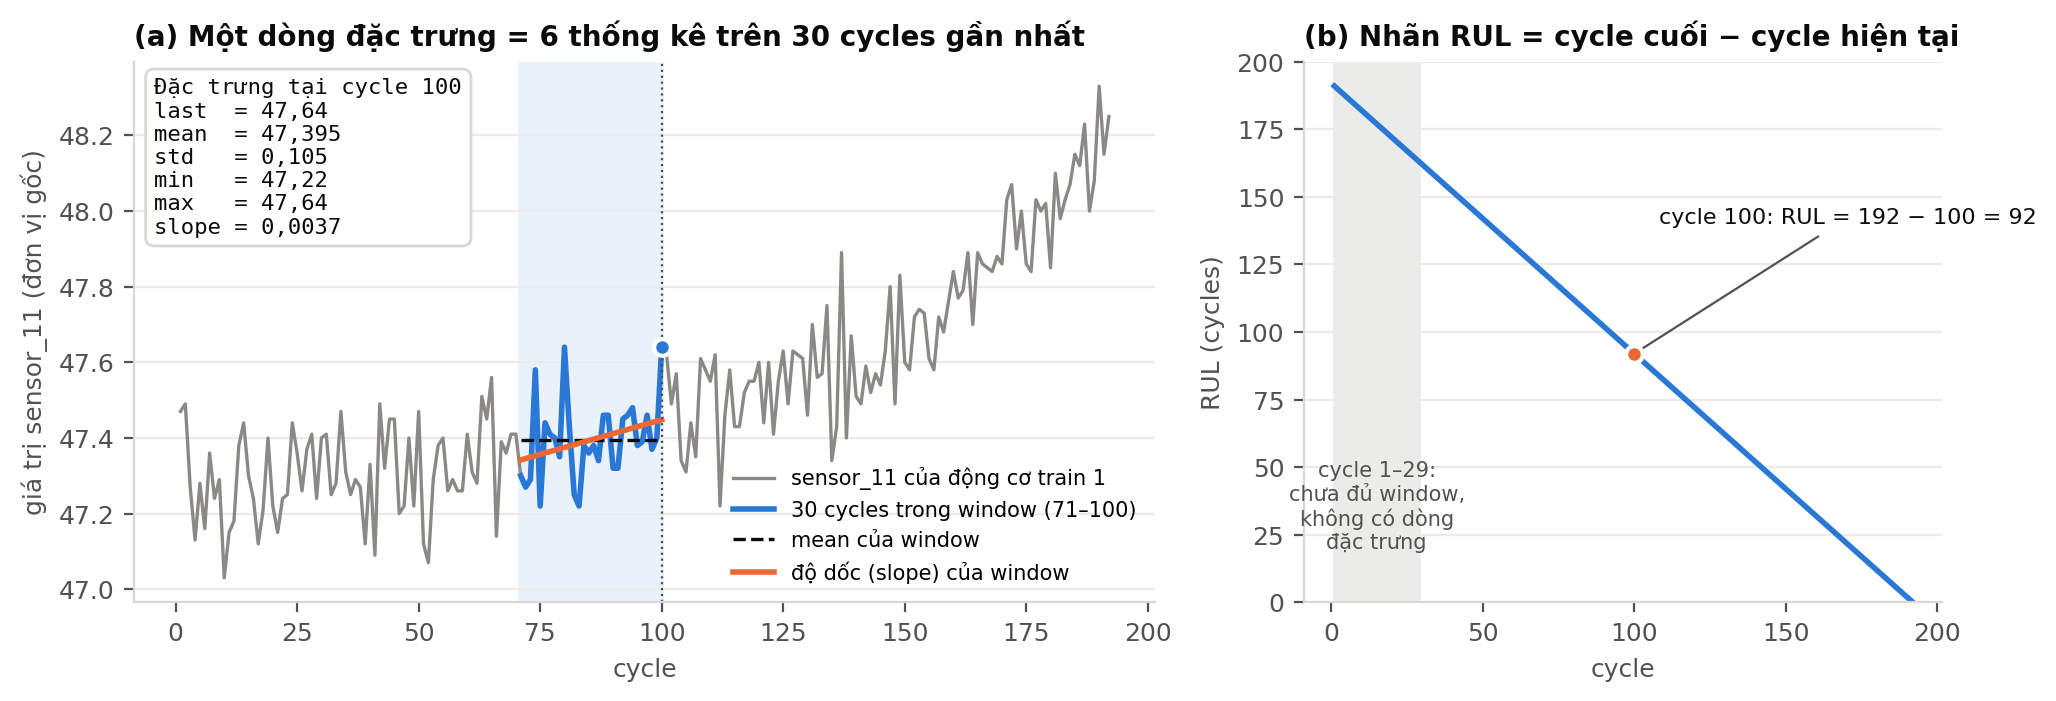
\includegraphics[width=\linewidth]{../outputs/diagnostics/figures/window_example.png}
\caption[Minh họa window và nhãn]{Minh họa bước tạo đặc trưng và nhãn trên train engine 1. (a) Sáu thống kê
của \texttt{sensor\_11} trên window cycles 71--100 tạo thành phần đặc trưng của dòng
cycle 100. (b) Nhãn RUL giảm tuyến tính về 0 tại cycle hỏng.}
\label{fig:window-example}
\end{figure}

ETL chỉ chuẩn hóa schema và kiểu dữ liệu, không scale giá trị sensor. Việc scale
chỉ diễn ra bên trong mô hình Ridge (StandardScaler fit trong từng fold) và khi tạo
Health Index; HGB dùng đặc trưng ở thang đo gốc.

Song song với sáu bước trên, nhánh phân tích tín hiệu làm mượt 14 sensor có xu
hướng bằng EWMA, rồi tạo Health Index cho mọi cycle
(Mục~\ref{sec:denoise-method}); nhánh này không cung cấp cột nào cho mô hình RUL.

Để kiểm tra tính đúng của ETL, PySpark thực hiện lại bước 1--5 và bộ đối chiếu so
sánh schema, khóa, số dòng và từng giá trị với kết quả Pandas. Benchmark đọc/ghi,
rolling features và đối chiếu Pandas--PySpark được trình bày ở
Mục~\ref{sec:res-etl}; dữ liệu nhân bản dùng cho benchmark không được dùng để huấn
luyện.

\subsection{Cột được dùng cho mô hình}
\label{sec:dp-columns}
Bảng~\ref{tab:column-roles} cho biết mỗi nhóm cột được dùng vào việc gì. Mô hình
chỉ nhận 126 cột đặc trưng, đặt tên theo mẫu \texttt{<sensor>\_\_<thống kê>}, ví dụ
\texttt{sensor\_11\_\_mean}. Ba cột khóa chỉ dùng để join và chia fold theo động
cơ. Ba operational settings không nằm trong tập đặc trưng: FD001 chỉ có một điều
kiện vận hành nên settings gần như không đổi; với FD002 và FD004, lựa chọn này trở
thành một giới hạn (Mục~\ref{sec:disc-transfer}).

\begin{table}[H]
\centering
\caption[Vai trò nhóm cột]{Vai trò của các nhóm cột.}
\label{tab:column-roles}
\small
\begin{tabularx}{\linewidth}{L{5.0cm} r X c}
\toprule
Nhóm cột & Số cột & Vai trò & Trong X? \\\midrule
\texttt{split}, \texttt{engine\_id}, \texttt{cycle} & 3 & Khóa: join, chia fold theo động cơ & Không \\
\texttt{setting\_1}--\texttt{setting\_3} & 3 & Điều kiện vận hành & Không \\
\texttt{sensor\_1}--\texttt{sensor\_21} & 21 & Tín hiệu gốc, dùng qua đặc trưng window; bản EWMA dùng cho Health Index & Không \\
\texttt{sensor\_k\_\_\{last, mean, std, min, max, slope\}} & 126 & Đặc trưng window 30 cycles & Có \\
\texttt{rul} & 1 & Nhãn (biến mục tiêu $y$) & Là $y$ \\
\bottomrule
\end{tabularx}
\end{table}

Báo cáo không thực hiện chọn lọc đặc trưng (feature selection): toàn bộ 126 cột
được giữ, kể cả các cột sinh ra từ sensor hằng. Cách làm này tránh dùng kết quả
EDA hoặc p-value trên toàn bộ train để chọn cột, vốn là một dạng data leakage đối
với cross-validation.

\subsection{Quan hệ giữa các bảng}
\label{sec:dp-relations}
Hình~\ref{fig:data-relations} và Bảng~\ref{tab:data-relations} mô tả quan hệ giữa
các bảng. Quan hệ duy nhất có bậc nhiều là giữa động cơ và quan sát (\textbf{1:N}):
một động cơ có từ 31 đến 362 cycles. Các quan hệ còn lại là \textbf{1:1} hoặc
\textbf{1:0..1}. Mỗi quan hệ được kiểm tra trực tiếp trên dữ liệu trong notebook
walkthrough; kết quả ghi ở cột cuối của bảng.

\begin{figure}[H]
\centering
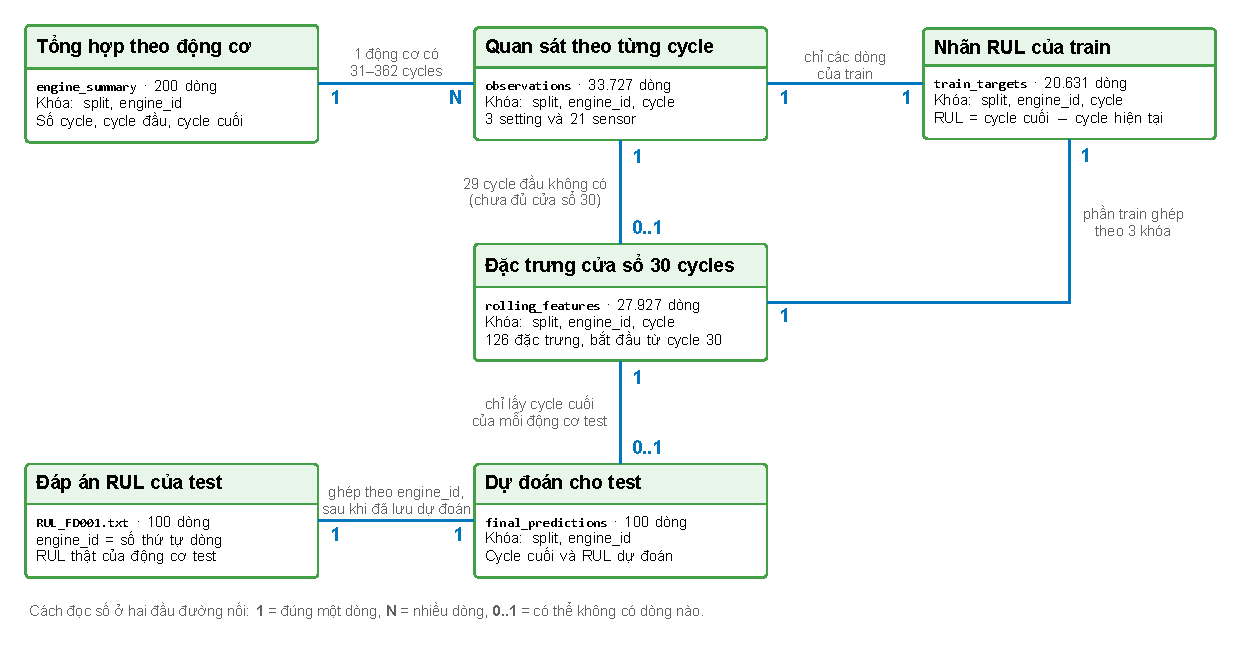
\includegraphics[width=\linewidth]{figures/data-relations.pdf}
\caption[Quan hệ giữa các bảng]{Quan hệ giữa các bảng trong một subset. Số ở hai đầu mỗi đường là bậc
quan hệ; ``0..1'' nghĩa là một dòng bên kia có thể có hoặc không có dòng tương ứng.}
\label{fig:data-relations}
\end{figure}

\begin{table}[H]
\centering
\caption[Kiểm tra quan hệ bảng]{Quan hệ giữa các bảng và kết quả kiểm tra trên FD001.}
\label{tab:data-relations}
\small
\begin{tabularx}{\linewidth}{L{4.4cm} c X}
\toprule
Hai bảng & Quan hệ & Kiểm tra trên dữ liệu \\\midrule
engine\_summary -- observations & 1 : N & Mỗi động cơ có 31--362 cycles \\
observations (train) -- train\_targets & 1 : 1 & 20.631 / 20.631 dòng khớp khóa \\
observations -- rolling\_features & 1 : 0..1 & 27.927 dòng có đặc trưng; 5.800 dòng (29 cycle đầu $\times$ 200 động cơ) không có \\
rolling\_features (train) -- train\_targets & 1 : 1 & 17.731 dòng sau join, đúng bằng số dòng đặc trưng train \\
final\_predictions -- test\_labels & 1 : 1 & 100 dòng, 100 động cơ test khác nhau \\
\bottomrule
\end{tabularx}
\end{table}

\textbf{Không có quan hệ nhiều-nhiều.} Một window dùng 30 quan sát, và hai window
liên tiếp dùng chung 29 quan sát. Đây là phụ thuộc theo thời gian khi tính toán,
không phải một phép join nhiều-nhiều giữa hai bảng: mỗi dòng đặc trưng vẫn gắn với
đúng một cycle cuối của window.

Việc join đúng khóa quan trọng vì một lỗi nhỏ có thể làm nhân số dòng. Với train
engine 1 (163 dòng đặc trưng, 192 dòng nhãn), join chỉ theo \texttt{engine\_id}
ghép mọi dòng đặc trưng với mọi dòng nhãn, tạo ra $163\times192=31.296$ dòng; join
theo đủ ba khóa trả về đúng 163 dòng. SQLite chưa khai báo ràng buộc khóa ngoại
(foreign key); thay vào đó, code kiểm tra quan hệ một-một bằng tham số
\texttt{validate="one\_to\_one"} và dừng nếu vi phạm.
